\qquad A seguir são apresentados os resultados obtidos na execução do algoritmo \textit{Merge Sort}.

% --- IMAGEM DA TABELA DO MERGE SORT ---
\begin{figure}[h!]
    \centering
    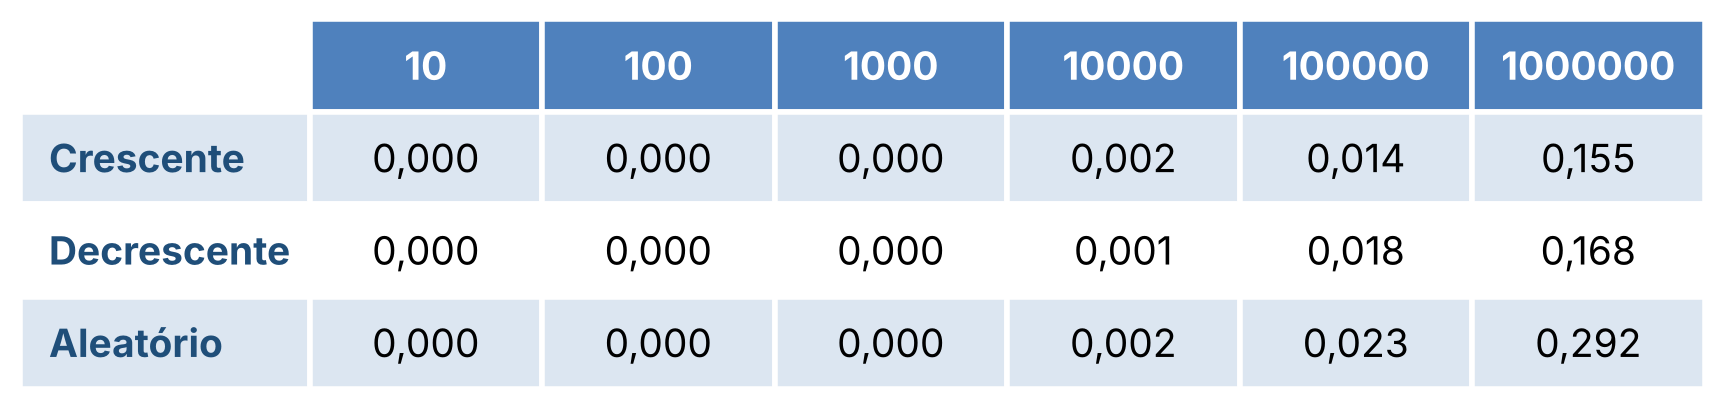
\includegraphics[width=1.0\textwidth]{Imagens/Merge Sort/tabela_merge.png}
    \caption{Tabela de tempo de execução (em segundos) do \textit{Merge Sort} (elaborado pelo autor).}
    \label{fig:tabela_merge}
\end{figure}

% --- IMAGEM DO GRÁFICO DO MERGE SORT ---
\begin{figure}[h!]
    \centering
    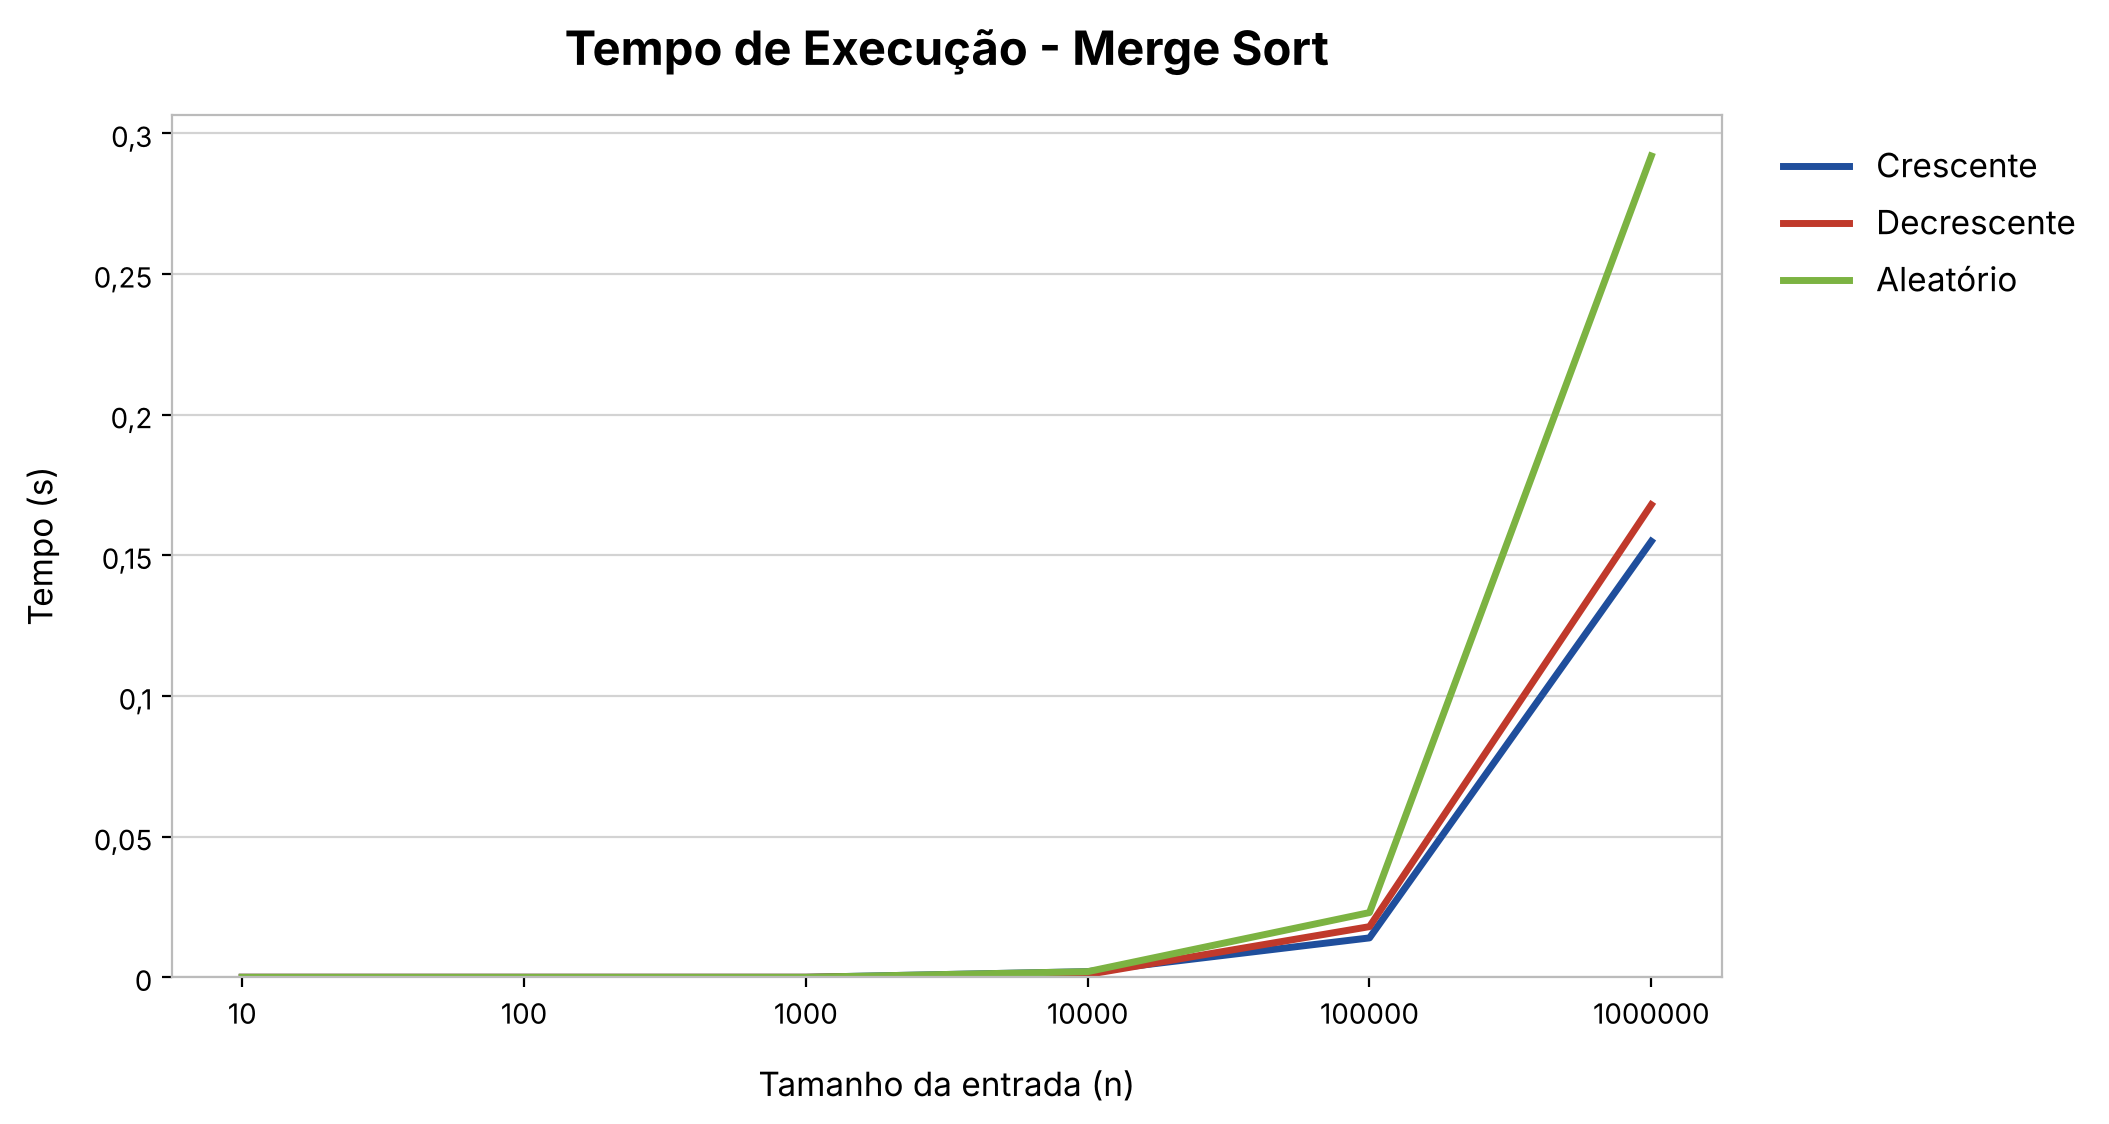
\includegraphics[width=1.0\textwidth]{Imagens/Merge Sort/grafico_merge.png}
    \caption{Desempenho do Algoritmo \textit{Merge Sort} (elaborado pelo autor).}
    \label{fig:grafico_merge}
\end{figure}

% --- ANÁLISE DOS RESULTADOS DO MERGE SORT ---

\qquad Os dados da Figura \ref{fig:tabela_merge} e o gráfico da Figura \ref{fig:grafico_merge} mostram que o \textit{Merge Sort} manteve tempos muito baixos em todos os cenários. Para as entradas de 10, 100 e 1.000 elementos, os tempos registrados foram de 0,000 segundo, o que indica apenas que a duração ficou abaixo da precisão do relógio utilizado. Diferenças só passam a ser perceptíveis a partir de 10.000 elementos.

\begin{itemize}
    \item \textbf{Desempenho em relação aos algoritmos quadráticos:} para ordenar um milhão de elementos no cenário aleatório, o \textit{Merge Sort} levou 0,292 segundo, enquanto o \textit{Selection Sort} levou 1.658,270 segundos e o \textit{Bubble Sort}, 3.954,730 segundos. Isso representa um desempenho cerca de 5.700 e 13.500 vezes superior, respectivamente.

    \item \textbf{Crescimento dos tempos:} ao passar de 100.000 para 1.000.000 de elementos, entrada dez vezes maior, o tempo do caso aleatório passou de 0,023 s para 0,292 s, um crescimento de aproximadamente 12,7 vezes. Esse valor é próximo do esperado para $n \log n$, que é de cerca de 12 vezes, e muito inferior às 100 vezes esperadas para um algoritmo quadrático. Os cenários crescente e decrescente cresceram cerca de 11 e 9 vezes, respectivamente.

    \item \textbf{Influência da ordem inicial:} diferente dos algoritmos quadráticos, a ordem dos dados teve pouco efeito sobre o desempenho. Para um milhão de elementos, os tempos foram de 0,155 s (crescente), 0,168 s (decrescente) e 0,292 s (aleatório). Isso é coerente com a análise teórica, segundo a qual o algoritmo realiza o mesmo número de divisões e intercalações em qualquer ordem. O cenário aleatório foi o mais lento, o que provavelmente se deve ao comportamento do processador, pois em entradas ordenadas as comparações da intercalação seguem um padrão previsível.
\end{itemize}

\qquad Em comparação com o \textit{Shell Sort}, o \textit{Merge Sort} foi mais rápido no cenário aleatório (0,292 s contra 0,461 s para um milhão de elementos), mas foi mais lento nos cenários crescente (0,155 s contra 0,099 s) e decrescente (0,168 s contra 0,129 s). Isso acontece porque o \textit{Shell Sort} aproveita a ordenação prévia dos dados, enquanto o \textit{Merge Sort} sempre executa todas as divisões e intercalações e ainda copia os elementos para o vetor auxiliar.

\qquad Os resultados mostram que o \textit{Merge Sort} é o algoritmo mais regular entre os estudados, com desempenho previsível e tempos inferiores a meio segundo para um milhão de elementos. Em contrapartida, ele exige memória adicional proporcional ao tamanho da entrada, o que o diferencia dos demais algoritmos deste trabalho.

\FloatBarrier